\documentclass[logo,reportComp]{thesis}
\usepackage[cpp,pseudo,linenum]{mypackage}

% https://tex.stackexchange.com/questions/227639/redefine-emph-to-be-both-bold-and-italic
\let\emph\relax % there's no \RedeclareTextFontCommand
\DeclareTextFontCommand{\emph}{\kaiti}

\title{分布式系统期末大作业}
\subtitle{分布式并发图系统}
\school{数据科学与计算机学院}
\author{陈鸿峥}
\classname{17大数据与人工智能}
\stunum{17341015}
\headercontext{分布式系统期末大作业}

\begin{document}

\maketitle

由于这一年刚好在做并行分布式大数据系统的相关工作,因此本次大作业我选择了自选题目,主要内容是\textbf{并发图系统}。
去年并行课上我已经实现了单机共享内存版本,而此次则将其扩展至多机分布式系统。
本文成果已以第一作者身份投稿至CCF-A类会议Annual Technical Conference (ATC'20),目前在审,详情可见补充材料。

两个版本的并发图系统都已开源,也可以在Github上查看我的提交记录。
系统核心代码采用C++进行编写,并使用OpenMP、Cilk Plus、MPI等多种并行编程框架,同时涉及模板元编程等C++11特性。
单机版本\footnote{Krill单机共享内存版本:\url{https://github.com/chhzh123/Krill}}总代码修改量超过1万行,分布式版本\footnote{Krill分布式版本:\url{https://github.com/chhzh123/GeminiGraph}}由于在单机版本上进行扩展,因此大约在3千行代码的修改量。

本实验报告将简要介绍本项目的背景与方法,并着重说明与本门课程的联系。
本项目与课程内容章节的对照可参见附录\ref{appendix:course}。

\section{简介}
图结构可以对大量现实世界中的复杂关系进行建模,因此近年来在社交网络、机器学习、科学计算等领域被广泛应用。
为了高效地处理这些超大规模的图结构,人们提出了很多图计算系统,从最早年谷歌由MapReduce延伸出来的Pregel~\cite{malewicz:pregel_icmd_2010},到之后在Spark上搭建的的GraphX~\cite{gonzalez:graphx_osdi_2014},再到现在在Facebook内部应用的Giraph~\cite{ching:giraph_vldb_2015}。
图计算系统经历了几个发展阶段,也一直是并行分布式计算领域一个极具挑战性的研究方向。

而随着越来越多应用在同一个大图上运行,并发图任务的需求也越来越大。
第一方面来源于\textbf{客户端-服务器的场景}。
类比传统的关系型数据库,多个用户可以同时对其发起请求。
对于图计算系统来说也是类似,很多可能在同一时间段内有多个用户在上面进行计算。
可能有些用户会关心一个大的社交网络内的人与人之间的$n$度关系(即子图匹配),而另一些用户关心哪些人可以构成一个具有一定共性的群体(即社群检测)。
这时如果这些用户同时发起请求,则要求系统快速地对这些查询作出应答。

而第二方面则来源于\textbf{对图应用的观察}。
我们发现事实上有大量的图应用都是由基本的图算法构成,而在该应用下同时执行这些算法就显得至关重要。
举一个最近的例子,图嵌入(graph embedding)是目前自然语言处理、推荐系统等方向一个非常重要的技术,其中采用的DeepWalk~\cite{perozzi:deepwalk_kdd_2014}、Node2Vec~\cite{grover_node2vec_2016}等随机游走的方法实际上就是在图上同时做多个$n$度的遍历,如何快速地对这些路径进行采样就成为了至关重要的问题。
这里的每一个遍历都可以看作是一个图计算任务(task),而这些图计算任务构成了一个完整的工作(job),即随机游走。
SOSP'19上已经有相关工作KnightKing~\cite{yang_knightking:_2019},但他们仅仅对随机游走本身进行并行优化,而我们则着重于更加通用的并发图计算任务。

目前的图计算系统大多都是为单一图计算任务而设计~\cite{shun:ligra_ppopp_2013,sundaram:graphmat_vldb_2015,pingali:galois_ppaa_2014,malewicz:pregel_icmd_2010,ching:giraph_vldb_2015,low:graphlab_vldb_2012},它们在任务内的并行已经发挥得非常出色,但对于这一最大粒度的并行——任务间并行——其实做得并不是很好,而主要原因来源于它们忽略了大量的共享关系,如共享的图结构、共享的访问顶点及共享的遍历模式等。

因此,在本项目中,我们提出了Krill这一并发图计算系统。
通过最大程度挖掘任务与任务之间的相互关系,利用\emph{图核融合}(graph kernel fusion)技术,减少冗余数据访问;同时提出了\emph{快速边界筛}和\emph{提前任务筛}来加速每轮迭代中的遍历。
Krill的单机共享内存版本基于Ligra~\cite{shun:ligra_ppopp_2013}搭建,而分布式的版本则基于陈文光老师的Gemini~\cite{zhu:gemini_osdi_2016}进行搭建。
最终,Krill比基准Ligra系统减少了14倍的内存访问开销,运行时间比其快8倍;分布式版本比当前最好的并发图计算系统Seraph~\cite{xue:seraph_hpdc_2014}快了4.25倍。

\section{背景与动机}
目前的图计算系统基本采用以下两种引擎,一种是Push的,即从源结点到汇结点进行遍历;另一种是Pull的,即从汇结点到源节点进行遍历。
两种方式各有优劣,而Krill采用了混合引擎以最大化这两者的优势。
\begin{center}
\begin{minipage}{0.45\linewidth}
\centering \textbf{Push Engine}
\begin{lstlisting}
parallel_for (vSrc : vertices) {
  if (!vSrc in frontier)
    continue;
  for (vDst : vSrc.outngh) {
    if (cond(vDst))
      atomicUpdate(vDst);
  }
}
\end{lstlisting}
\end{minipage}\hfill
\begin{minipage}{0.45\linewidth}
\centering \textbf{Pull Engine}
\begin{lstlisting}
parallel_for (vDst : vertices) {
  if (!cond(vDst))
    continue;
  for (vSrc : vDst.inngh) {
    if (vSrc in frontier)
      update(vDst);
  }
}
\end{lstlisting}
\end{minipage}
\end{center}

在数据结构表示上,图数据可以被分割成两个部分,一部分是图结构,即图的邻接关系;另一部分为图性质,即图上每一顶点的专有数据。
通常图结构采用稀疏压缩行(Compressed Sparse Row, CSR)格式存储,而图性质则采用一般的数组进行存储,如图\ref{fig:data_structure}所示。
\begin{figure}[H]
\centering
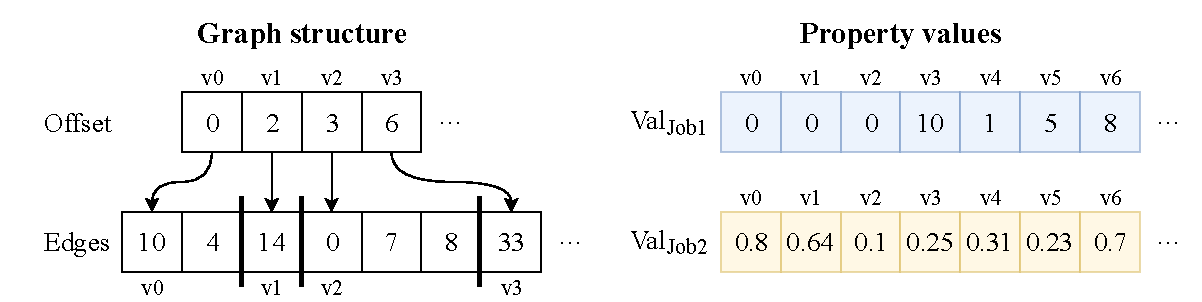
\includegraphics[width=0.8\linewidth]{fig/krill-Data-structure.pdf}
\caption{图结构与图性质}
\label{fig:data_structure}
\end{figure}

近几年已经有北大代亚非老师组的Seraph~\cite{xue:seraph_hpdc_2014}和华中科技大学金海老师组的CGraph~\cite{zhang:cgraph:_2018}两个并发图系统被研发,但是仍存在大量的性能提升空间,包括以下三点:
\begin{itemize}
	\item \textbf{不同任务之间的相互关系}:由于Seraph和CGraph将每一个任务都看作是独立的个体,因此丧失了对它们统一表示及统一优化的机会。Krill则提出了图核融合技术,将所有的任务看作一个整体进行处理,进而可以充分挖掘任务之间的相似性,以减少不必要的访问计算开销。
	\item \textbf{大量的内存冗余访问}:对于Seraph和CGraph来说,由于每个任务都是独立的个体,因此在一轮迭代中,总的访问图结构的时间为$O(c|E|)$,其中$c$为任务数量,$|E|$为图中边数。
	事实上,如果我们将这些任务看成一个整体,统一去访问图结构,那么访问开销将会被降至$O(|E|)$,这也是图核融合的核心思想。
	\item \textbf{未利用的大量内存带宽}:随着近年来体系结构和图处理技术的发展,IO开销被降低,伴随着就是大量的内存访问带宽被闲置。我们通过实验数据得到,单一任务下内存带宽的利用率最大仅到80\%,且大多数情况远低于这个水平。
	但如果简单地将这些任务进行并行,那么必然会导致带宽互相侵占,进而各个任务的性能降低。
	因此需要有更加好的任务管理方案,来充分利用这些带宽资源。
\end{itemize}

\section{核心技术}
这一节将简要叙述Krill中所采用的核心技术,详情细节请见原始论文。

\subsection{图核融合}
所谓图核(graph kernel),即一个计算任务,可以类比于GPU的计算核。
考虑图$G(V,E)$,则图核是一个$f:V\times V\mapsto\rr$的映射,可以标识一个图任务。
当多个图任务$f_1,\ldots,f_k$在一起考虑时,我们希望找到这样的映射$g$使得
\begin{align}
g&=f_1\times f_2\times\cdots\times f_k\\
g&:V\times V\mapsto\rr
\end{align}
此即图核融合的最核心思想:用一个计算核代替所有计算核,其计算效果跟所有计算核同时计算的效果等效,这样便能减少不必要的内存访问开销。

具体实现上则是由上文的观察,将遍历任务的循环体内移,使得原来$O(c|E|)$次的图结构访问,下降至$O(|E|)$次。
对应的Push和Pull引擎可见算法\ref{alg:push_kerf}和算法\ref{alg:pull_kerf}。
\begin{algorithm}[!ht]
\caption{结合图核融合的Push引擎}
\label{alg:push_kerf}
\begin{algorithmic}[1]
\For{\textbf{each} vSrc \textbf{in} vertices}
\For{vDst \textbf{in} vSrc.outngh}
\For{\textbf{each} job \textbf{in} jobList}
\State condPushUpdate(job,vSrc,vDst)
\EndFor
\EndFor
\EndFor
\end{algorithmic}
\end{algorithm}
\begin{algorithm}[!ht]
\caption{结合图核融合的Pull引擎}
\label{alg:pull_kerf}
\begin{algorithmic}[1]
\For{\textbf{each} vDst \textbf{in} vertices}
\For{vSrc \textbf{in} vDst.inngh}
\For{\textbf{each} job \textbf{in} jobList}
\State condPullUpdate(job,vSrc,vDst)
\EndFor
\EndFor
\EndFor
\end{algorithmic}
\end{algorithm}

其中的\verb'condPushUpdate'和\verb'condPullUpdate'则是顶点更新规则,包括判断源节点是否是活跃结点、目标结点是否满足更新前提、目标结点是否被更新函数更新。

\subsection{快速边界筛}
可以看到,如果仅采用前文所述的简单图核融合引擎,那么依然存在大量的冗余遍历,一方面是源节点的访问冗余,另一方面则是汇结点的访问冗余。

考虑源结点的情况,即Push引擎。
其实在单任务图系统上Push的方式已经做得非常成熟,常常利用边界集(frontier)优化的方法来加速遍历\cite{shun:ligra_ppopp_2013,zhu:gemini_osdi_2016},因此Krill同样采用边界集来跟踪每一轮迭代中的活跃结点。

如果设$k$个任务的边界集分别为$\mD_1,\mD_2,\ldots,\mD_k$,则
\begin{equation}
\mD_\cup=\bigcup_{i=1}^k\mD_i=\mD_1\cup\mD_2\cdots\cup\mD_k
\end{equation}
必然是包括这些边界集中所有顶点的最小集合,这一点利用简单的集合论知识可以证明。

那么对于每一个任务$i$,只需维护自己的边界集$\mD_i$;对于Krill系统,则只需在此基础上维护一个公共边界集$\mD_\cup$即可做到活跃结点的快速筛选,核心伪代码如算法\ref{alg:push_fff}所示。
\begin{algorithm}[htbp]
\caption{添加了快速边界筛的Push引擎}
\label{alg:push_fff}
\begin{algorithmic}[1]
\For{\textbf{each} vSrc \textbf{in} currCommonFrontier}
\For{vDst \textbf{in} vSrc.outngh}
\For{\textbf{each} job \textbf{in} jobList}
\State job.condPushUpdateFFF\\\qquad\qquad\qquad(CommonFrontier,vSrc,vDst)
\EndFor
\EndFor
\EndFor
\end{algorithmic}
\end{algorithm}

其中的\verb'condPushUpdateFFF'与算法\ref{alg:push_kerf}的类似,只是添加了更新公共边界集的步骤。

\subsection{提前任务筛}
对于Pull引擎来说,由于外层循环先遍历汇结点,内层循环再遍历源节点,因此无法充分利用边界集优化技术,需要考虑其他方式来减少对结点的冗余访问。

Krill选择在进入内层循环之前,提前对需要遍历源节点的任务给筛选出来,然后在内层循环才对这些任务进行遍历,核心伪代码如算法\ref{alg:pull_atf}所示。
\begin{algorithm}[htbp]
\caption{添加了提前任务筛的Pull引擎}
\label{alg:pull_atf}
\begin{algorithmic}[1]
\For{\textbf{each} vDst \textbf{in} vertices}
\State availJob.initialize()
\For{\textbf{each} job \textbf{in} jobList}
\If{job.cond(vDst)}
\State availJob.append(job)
\EndIf
\EndFor
\State{\textbf{if} (availJob.empty())  \textbf{continue}}
\For{vSrc \textbf{in} vDst.inngh}
\For{\textbf{each} job \textbf{in} availJob}
\State job.condPullUpdateAJF(vSrc,vDst)
\If{(!job.cond(vDst))}
\State availJob.del(job)
\EndIf
\EndFor
\EndFor
\EndFor
\end{algorithmic}
\end{algorithm}

其中的\verb'condPullUpdateAJF'与算法\ref{alg:pull_kerf}的类似,同样添加了更新公共边界集的流程。

\section{系统实现}
Krill的执行流程如图\ref{fig:overview}所示。
Krill主要包括了一个提取器(fetcher)、一个调度器(scheduler)和一个执行器(executor)。
当有新的任务到来时,提取器将会抓取任务并将其添加入任务池中。
在每一轮迭代开始时,调度器会将正在进行的任务和新的任务重新进行融合,然后将融合后的任务交给执行器去执行。
\begin{figure}[H]
\centering
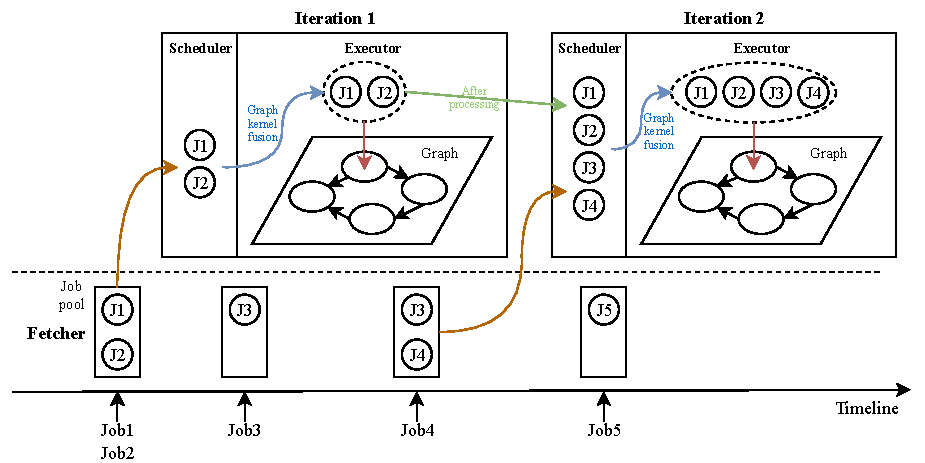
\includegraphics[width=0.8\linewidth]{fig/krill-interactive.pdf}
\caption{Krill的执行流程}
\label{fig:overview}
\end{figure}

我们采用OOP对任务进行封装,为每一个任务提供一个基类(base class),同时提供一个容器类\verb'Kernels',可以将所有的任务封装在里面。
用户只需在每个任务内定义基本的\verb'cond'、\verb'update'\\
和\verb'updateAtomic'函数,并将这些任务打包在\verb'Kernels'类中,通过\verb'setKernels'函数即可将任务传递给Krill系统进行执行。
用户API样例如下:
\begin{lstlisting}
void setKernels(graph& G, Kernels& K)
{
  BFS* bfs = new BFS(G.n); // pass in # of vertices
  SSSP* sssp = new SSSP(G.n);
  K.appendJob({bfs,sssp});
}
\end{lstlisting}


\section{实验}
这里主要讲述Krill分布式的部分,也是本次项目的重点,其单机共享内存的实验方式与结果可以见原始论文。

我选择了陈文光老师组的Gemini~\cite{zhu:gemini_osdi_2016}系统进行扩展实现。
Gemini是\textbf{分布式图计算系统}的典范,但其依然是单任务图计算系统,因此我将其扩展为支持并发图任务,同时在上面实现我的Krill系统及现有的并发图Seraph~\cite{xue:seraph_hpdc_2014}系统。

\subsection{Seraph实现}
要实现并发图处理,很关键一点在于\textbf{将图结构与图性质解耦}(decouple)。
原本的Gemini将关于图的所有数据都封装在一个类\verb'Graph'中,包括分布式节点的通信缓存(buffer)也封装在其中,这直接导致一个图只能对应一个任务,而无法在同一个图上执行多个任务。

因此使Gemini能够支持并发图处理的第一步操作就是解耦,将图结构封装在原始的\verb'Graph'类中,而图性质及其他相关数据则新建其他的类进行存储,同时通过传递参数的方式实现调用。
解耦后的计算模式如图\ref{fig:ges}所示,即Seraph~\cite{xue:seraph_hpdc_2014}提出来的Graph-State-Exchange data (GES)计算模式。
采用这种方法即可以方便地对图结构和图性质分开处理,用户只需关心图性质的处理逻辑,而关于图结构的遍历则全部交由图计算系统完成。
\begin{figure}[H]
\centering
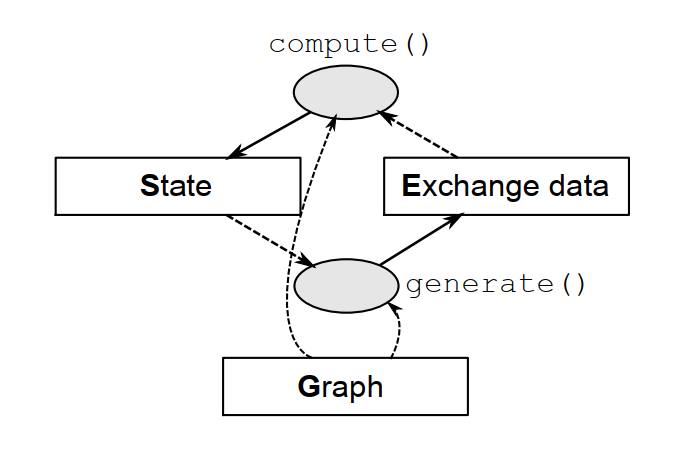
\includegraphics[width=0.6\linewidth]{fig/GES.png}
\caption{Graph-State-Exchange data (GES)计算模式}
\label{fig:ges}
\end{figure}

解耦完图结构和图性质后,就可以在同一个图上进行多个任务的操作。
为实现Seraph,采用C++11的线程库\verb'<thread>',为每个任务分配一个线程,然后共享相同的图结构,而图性质则依不同任务而不同,它们通信缓存也相互不同,以标号的形式避免冲突。

注意这里图结构的读入与划分(partition)是由Gemini完成的,它保证了在每一个分布式节点上都存在一部分的图划分。
但由于每一个节点都没有全部的图数据,因此在具体实现算法时需要确保任务的图性质数据都正常在节点之间传递,这一步需要在算法中用\verb'emit'强制声明。

\subsection{Krill实现}
Gemini系统提供的用户API相对比较底层,核心为\verb'process_edges'函数,其定义如下
\begin{lstlisting}
template<typename R, typename M>
R process_edges(
	std::function<void(VertexId)> sparse_signal,
	std::function<R(VertexId, M, VertexAdjList<EdgeData>)> sparse_slot,
	std::function<void(VertexId, VertexAdjList<EdgeData>)> dense_signal,
	std::function<R(VertexId, M)> dense_slot,
	Bitmap * active
	)
\end{lstlisting}

其中四个用户自定义函数对应着其Signal-Slot的编程模型,如图\ref{fig:signal-slot}所示,其声明了每个图顶点的更新方式,以及在分布式环境下如何在Master和Mirror之间传递数据。
\begin{figure}[H]
\centering
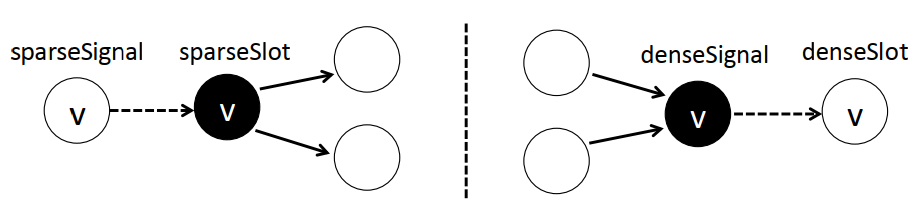
\includegraphics[width=0.8\linewidth]{fig/signal-slot.png}
\caption{Sparse-dense signal-slot模型}
\label{fig:signal-slot}
\end{figure}

为实现Krill的几个技术点,我们其实只需更改用户自定义的四个函数即可。
\begin{itemize}
\item 通过将任务遍历的循环移至最里层,可以实现\textbf{图核融合}。
\item 通过新建\verb'common_active_in/out'数组,实时维护公共边界集,实现\textbf{快速边界筛}。
\item 通过在\verb'dense_signal'开始部分先轮询任务数组,判断更新前提条件,并创建位掩码(bitmask)进行维护,即可实现\textbf{提前任务筛}。
\end{itemize}

由于现在是多个图任务占用一个处理单元,因此在消息传递时需要对每个活跃结点的处所有任务的消息打包进行传递。
由于\verb'process_edges'的API参数均为模板,因此可以新建一个消息传递类(message passing class),类似gRPC的方式,提前组织好数据后再统一进行发送,这样也大大减少了分布式节点间的通信量。
完整实施样例可以见附录\ref{appendix:krill}。

\subsection{实验环境}
我们采用了宽度优先搜索(BFS)、连通分量(CC)、页面排序(PageRank)和单源最短路径(SSSP)四个算法作为基本的算法。
然后将这些算法分别组合成如表\ref{tab:job_sets}所示的任务集,每个任务集都由8个基本的算法组成。
其中的异构性和同构性是通过内存访问带宽大小来进行分类的,详情可见原始论文或文~\cite{pan:congra_iccd_2017}。
\begin{table}[H]
\centering
\caption{评测任务集描述}
\label{tab:job_sets}
\begin{tabular}{|c|c|c|}\hline
\textbf{任务集} & \textbf{算法} & \textbf{Description} \\\hline
Homo1 & $\{BFS,CC\}\times 4$ & 同构\\\hline
Homo2 & $\{PR,SSSP\}\times 4$ & 同构\\\hline
Heter & $\{BFS,CC,PR,SSSP\}\times 2$ & 异构 \\\hline
M-BFS & $\{BFS\}\times 8$ & 相同任务 \\\hline
M-SSSP & $\{SSSP\}\times 8$ & 相同任务 \\\hline
\end{tabular}
\end{table}

关于单机共享内存的评测请见原始论文,这里只给出分布式环境下评测所采用的两个数据集。
\begin{table}[H]
\centering
\caption{实验所采用的数据集}
\label{tab:dataset}
\begin{tabular}{|c|c|c|c|c|}\hline
\textbf{简写} & \textbf{数据集} & \textbf{$|V|$} & \textbf{$|E|$} & \textbf{大小}\\\hline
RM & rMat24~\cite{graph_500} & 33.6 M & 168 M & 2.0 GB\\\hline
TW & Twitter~\cite{yang:TW_wsdm_2011} & 41.7 M & 1.4 B & 15.7 GB\\\hline
\end{tabular}
\end{table}

由于超算机时占用严重,因此实验只在实验室的小集群上运行,环境配置请见原始论文。

运行时间实验结果如图\ref{fig:distributed}所示,可以清晰看到我们的Krill系统比Seraph系统最快快了4.25倍,这很大原因来源于Krill对各个图任务之间关系的挖掘。
\begin{figure}[H]
\centering
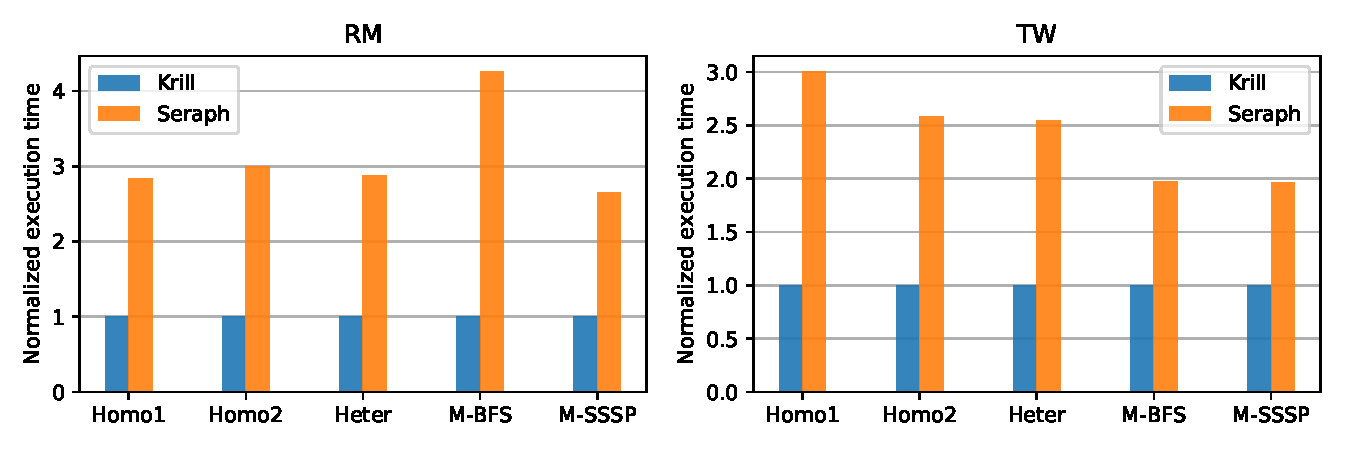
\includegraphics[width=0.9\linewidth]{fig/distributed.pdf}
\caption{分布式环境下Krill与Seraph运行时间比较}
\label{fig:distributed}
\end{figure}

内存访问量比较结果如表\ref{tab:memory}所示,从中也可以看出Krill减少了近1倍的内存访问开销,而且这还是在没有优化的情况下的比较,如果将Krill的所有优化技术全部结合使用上去,那么得出的内存访问减少量的差异应该更加明显。
\begin{table}[H]
\caption{Krill和Seraph内存访问量比较(RM)}
\label{tab:memory}
\begin{tabular}{cccccc}\hline
& \textbf{Homo1} & \textbf{Homo2} & \textbf{Heter} & \textbf{M-BFS} & \textbf{M-SSSP}\\\hline
Krill & 121,277,102,205 & 184,484,882,245 & 161,182,322,856 & 71,368,664,593 & 156,714,974,125\\
Seraph & 183,416,200,102 & 375,861,175,531 & 287,505,536,960 & 115,908,456,530 & 351,852,690,249\\\hline
\end{tabular}
\end{table}

\section{总结}
本项目陈述了并发图处理的重要性,并且提出了自己的并发图系统Krill,也给出了单机共享内存和分布式环境下的实现。
实验结果体现了我们提出的三个方法的有效性,大大减少了内存访问开销,进而提升了系统的整体性能。
我们也相信Krill能够处理更加复杂的并发图任务,并得到更加广泛的应用。

\bigskip
PS:这里为了说明Krill和Seraph的分布式系统实现确实是本次课程期间完成,且具有一定工作量,附上Github提交记录截图,chhzh123为我的Github账号。
\begin{figure}[H]
\centering
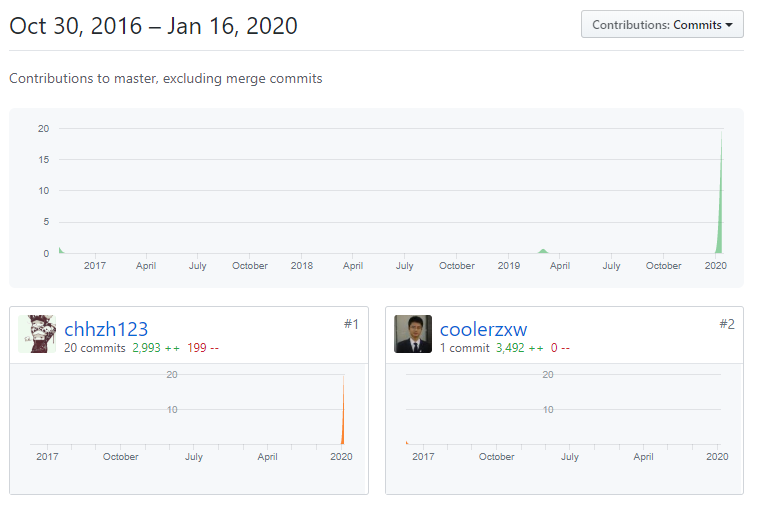
\includegraphics[width=0.8\linewidth]{fig/github.png}
\end{figure}

\bibliographystyle{unsrt}
\bibliography{ATC-2020}

\newpage
\appendixconfig
\appendix
\section{章节对照}
\label{appendix:course}
项目中所使用的技术与课程内容的关联性对照如下表所示,实际上分布式系统课程的内容是紧密渗透在我的项目之中的,毕竟图计算系统就是一个\textbf{物理分布,逻辑集中;个体独立,整体统一}的分布式系统。

\begin{center}
\begin{tabular}{ccc}\hline
\textbf{项目采用技术} & \textbf{课程章节} & \textbf{课程内容}\\\hline
类封装 & 第1章 & 透明性\\
图结构与图性质解耦 & 第1章 & 策略与机制相分离\\
多线程技术 & 第3章 & 线程\\
Master-Mirror消息打包通信 & 第4章 & RPC/gRPC\\
原子操作 & 第7章 & 以数据为中心的一致性模型\\
并行编程 & 第11章 & 大数据\\
VSCode + Github & 补充内容 & DevOps连续集成\\\hline
\end{tabular}
\end{center}

当然还有很多细节技术这里没有一一列举出来,总的来说在分布式系统这门课上我学习到了很多东西,同时也都能够学以致用。

\section{Gemini+Krill编程实例(Multi-BFS)}
\label{appendix:krill}
假设前期所有数据结构都准备好了,这里只展示最核心的遍历步骤及消息传递的数据结构,考虑8个BFS的并发图任务。
\begin{lstlisting}
class VecVertexId
{
public:
    VecVertexId() = default;
    VecVertexId(const VertexId val)
    {
        for (int i = 0; i < 8; ++i)
            vertex_id[i] = val;
    }
    VecVertexId(const VecVertexId &other)
    {
        for (int i = 0; i < 8; ++i)
            vertex_id[i] = other.vertex_id[i];
    }
    VertexId vertex_id[8] = {0};
};

active_vertices = graph->process_edges<VertexId, VecVertexId>(
    [&](VertexId src) {
        VecVertexId vecId(graph->vertices);
        for (int i = 0; i < 8; ++i)
            if (active_in[i]->get_bit(src))
                vecId.vertex_id[i] = src;
        graph->emit(src, vecId);
    },
    [&](VertexId src, VecVertexId msg, VertexAdjList<Empty> outgoing_adj) {
        VertexId activated = 0;
        for (AdjUnit<Empty> *ptr = outgoing_adj.begin; ptr != outgoing_adj.end; ptr++)
        {
            VertexId dst = ptr->neighbour;
            bool flag = false;
            for (int i = 0; i < 8; ++i)
            {
                if (active_in[i]->get_bit(src) && parent[i][dst] == graph->vertices && cas(&parent[i][dst], graph->vertices, msg.vertex_id[i])) // be careful!
                {
                    active_out[i]->set_bit(dst);
                    flag = true;
                }
            }
            if (flag)
            {
                activated += 1;
                common_active_out->set_bit(dst);
            }
        }
        return activated;
    },
    [&](VertexId dst, VertexAdjList<Empty> incoming_adj) {
        // advanced task filter
        // int bit_mask = 0;
        bool bit_mask[8] = {0};
        int cnt = 0;
        for (int i = 0; i < 8; ++i)
        {
            if (parent[i][dst] != graph->vertices) //(visited[i]->get_bit(dst))
            {
                // return;
                // bit_mask &= 1 << i;
                bit_mask[i] = 1;
                cnt++;
            }
        }
        if (cnt == 8)
            return; // all visited
        VecVertexId vecId(graph->vertices);
        bool flag = false;
        for (AdjUnit<Empty> *ptr = incoming_adj.begin; ptr != incoming_adj.end; ptr++)
        {
            VertexId src = ptr->neighbour;
            for (int i = 0; i < 8; ++i)
            {
                if (!bit_mask[i] && active_in[i]->get_bit(src)) // dst not visited & src active
                {
                    vecId.vertex_id[i] = src;
                    bit_mask[i] = 1;
                    flag = true;
                }
            }
        }
        if (flag)
            graph->emit(dst, vecId);
    },
    [&](VertexId dst, VecVertexId msg) {
        bool flag = false;
        for (int i = 0; i < 8; ++i)
        {
            if (cas(&parent[i][dst], graph->vertices, msg.vertex_id[i]))
            {
                active_out[i]->set_bit(dst);
                // return 1;
                flag = true;
            }
        }
        if (flag)
        {
            common_active_out->set_bit(dst);
            return 1;
        }
        else
            return 0;
    },
    common_active_in, nullptr);active_vertices = graph->process_edges<VertexId, VecVertexId>(
    [&](VertexId src) {
        VecVertexId vecId(graph->vertices);
        for (int i = 0; i < 8; ++i)
            if (active_in[i]->get_bit(src))
                vecId.vertex_id[i] = src;
        // VecVertexId vecId(src);
        graph->emit(src, vecId);
    },
    [&](VertexId src, VecVertexId msg, VertexAdjList<Empty> outgoing_adj) {
        VertexId activated = 0;
        for (AdjUnit<Empty> *ptr = outgoing_adj.begin; ptr != outgoing_adj.end; ptr++)
        {
            VertexId dst = ptr->neighbour;
            bool flag = false;
            for (int i = 0; i < 8; ++i)
            {
                if (active_in[i]->get_bit(src) && parent[i][dst] == graph->vertices && cas(&parent[i][dst], graph->vertices, msg.vertex_id[i])) // be careful!
                {
                    active_out[i]->set_bit(dst);
                    flag = true;
                }
            }
            if (flag)
            {
                activated += 1;
                common_active_out->set_bit(dst);
            }
        }
        return activated;
    },
    [&](VertexId dst, VertexAdjList<Empty> incoming_adj) {
        // advanced task filter
        // int bit_mask = 0;
        bool bit_mask[8] = {0};
        int cnt = 0;
        for (int i = 0; i < 8; ++i)
        {
            if (parent[i][dst] != graph->vertices) //(visited[i]->get_bit(dst))
            {
                // return;
                // bit_mask &= 1 << i;
                bit_mask[i] = 1;
                cnt++;
            }
        }
        if (cnt == 8)
            return; // all visited
        VecVertexId vecId(graph->vertices);
        bool flag = false;
        for (AdjUnit<Empty> *ptr = incoming_adj.begin; ptr != incoming_adj.end; ptr++)
        {
            VertexId src = ptr->neighbour;
            for (int i = 0; i < 8; ++i)
            {
                if (!bit_mask[i] && active_in[i]->get_bit(src)) // dst not visited & src active
                {
                    vecId.vertex_id[i] = src;
                    bit_mask[i] = 1;
                    flag = true;
                }
            }
        }
        if (flag)
            graph->emit(dst, vecId);
    },
    [&](VertexId dst, VecVertexId msg) {
        bool flag = false;
        for (int i = 0; i < 8; ++i)
        {
            if (cas(&parent[i][dst], graph->vertices, msg.vertex_id[i]))
            {
                active_out[i]->set_bit(dst);
                // return 1;
                flag = true;
            }
        }
        if (flag)
        {
            common_active_out->set_bit(dst);
            return 1;
        }
        else
            return 0;
    },
    common_active_in, nullptr);
\end{lstlisting}

\end{document}